% !TeX root = ../../main.tex
% DRAFT: not yet \input from 3_barcs-results.tex. Placement to be decided in review.
\subsection{A donor- and mouse-adjusted fit re-analyses an in vivo T cell IFN$\gamma$
screen}
\label{sec:liu}

We applied BARCS to an in vivo screen where between-animal variation, not
sequencing noise, is the dominant nuisance.  Supplementary Table~5 of
\citet{liu2026invivo} reports the focused sub-library arm of a
tumour-infiltrating T cell IFN$\gamma$ screen: 268 sgRNAs (36 genes at six
guides plus 52 non-targeting controls), with tumour-infiltrating T cells sorted
into the top-20\% IFN$\gamma^\text{high}$ and bottom-20\% IFN$\gamma^\text{low}$
gates.  It is the only screen in the study that publishes per-mouse counts.  Two
independent arms were run: CD3-scFv T cells against A375\textsuperscript{low}
tumours (Arm~A; 16 libraries, 8 mice, 3 donors) and NY-ESO-1 TCR T cells against
wild-type A375 (Arm~B; 8 libraries, 4 mice, 2 donors).  BARCS fitted one
guide-level sort-gate coefficient with donor indicators (\texttt{$\sim$ gate +
donor}) on each arm, and refitted Arm~A with mouse indicators
(\texttt{$\sim$ gate + mouse}) as a sensitivity analysis.  A positive coefficient
marks a knockout enriched among IFN$\gamma^\text{high}$ cells.  This is a
re-analysis of published median-normalised counts, not an independent
replication; the published analysis used a one-sided MAGeCK RRA test, which
collapses each contrast to a treatment-versus-control comparison and cannot carry
donor or mouse as explicit terms.

The fit was well behaved on Arm~A.  Of 268 guides, 267 produced finite fits, all
converged, none reached the dispersion boundary, and the median extra-binomial
$\rho$ was $1.22\times10^{-4}$.  The 52 non-targeting controls behaved as a
proper null: fitted as a single pseudo-gene they gave effect $-0.019$
($p=0.26$, FDR $0.63$), and the control-tail calibration factor was exactly
$1.00$, so no correction was applied.  The screen's built-in positive controls
were the two strongest signals in the correct direction --- \textit{IFNG}
($-0.538$, FDR $1.6\times10^{-4}$, 6/6 guides agreeing) and \textit{TNF}
($-0.266$, FDR $2.1\times10^{-4}$, 6/6 guides).

BARCS reproduced the published biology.  Six genes reached FDR $<0.10$ in Arm~A,
all in the enriched direction: \textit{MED12}, \textit{STT3B}, and
\textit{TNFAIP3} (each FDR $0.008$), \textit{NFKBIA} ($0.074$), \textit{GNAS}
($0.087$), and \textit{RASA2} ($0.098$).  Gene-level effects agreed with the
published MAGeCK log$_2$ fold changes at Spearman $\rho=0.90$ (Arm~A) and $0.92$
(Arm~B), and the two independent arms agreed with each other at Pearson
$r=0.72$ ($p=6\times10^{-7}$, 36 genes), with 9/9 sign agreement among genes
reaching FDR $<0.10$ in either arm (Figure~\ref{fig:liu}).  Both targets the
authors prioritised reappeared in the arm where the paper found each strongest:
\textit{GNAS} in Arm~A and \textit{STUB1} in Arm~B ($0.048$).  Recovery is not
validation: of these genes, only \textit{GNAS} and \textit{STUB1} were
individually knocked out and tested by \citet{liu2026invivo}; the others are
consistent-direction screen evidence, with \textit{TNFAIP3} and \textit{RASA2}
established by earlier work.

The design matrix is the point of difference.  Because both sort gates come from
the same animal, mouse is the natural pairing factor.  Refitting Arm~A as
\texttt{$\sim$ gate + mouse} spent degrees of freedom (12 to 7) but lowered the
median $\rho$ to $8.42\times10^{-5}$ and raised guide-level discoveries from 7 to
21 (Table~\ref{tab:liu}).  \textit{TNFAIP3} and \textit{RASA2} strengthened
(FDR $0.008\to0.001$ and $0.098\to0.025$), and both are supported independently
by Arm~B.  A one-sided RRA test on the same two gates cannot absorb this
between-mouse structure, because it has no term for it.

\begin{table}[htbp]
\centering
\caption{Arm~A donor- versus mouse-paired fits.  Gene FDRs under the primary
\texttt{$\sim$ gate + donor} model, the \texttt{$\sim$ gate + mouse} sensitivity
model, and the independent Arm~B \texttt{$\sim$ gate + donor} fit.  BARCS effects
are logit-scale coefficients; a positive value marks enrichment among
IFN$\gamma^\text{high}$ cells.  \textit{NTCTRL} is the pooled non-targeting
control pseudo-gene.}
\label{tab:liu}
\small
\setlength{\tabcolsep}{6pt}
\begin{tabular}{lrrrl}
\toprule
Gene & Effect & \texttt{+ donor} & \texttt{+ mouse} & Arm~B\\
\midrule
\textit{TNFAIP3} & $+0.228$ & $0.008$ & $0.001$ & $0.004$\\
\textit{RASA2}   & $+0.262$ & $0.098$ & $0.025$ & $8.1\times10^{-4}$\\
\textit{NFKBIA}  & $+0.251$ & $0.074$ & $0.031$ & $0.038$\\
\textit{MED12}   & $+0.246$ & $0.008$ & $0.036$ & $0.647$\\
\textit{STT3B}   & $+0.247$ & $0.008$ & $0.025$ & $0.487$\\
\textit{GNAS}    & $+0.204$ & $0.087$ & $0.105$ & $0.208$\\
\textit{P2RY8}   & $-0.105$ & $0.109$ & $0.555$ & $0.881$\\
\textit{PTGER4}  & $+0.149$ & $0.109$ & $0.496$ & $0.881$\\
\textit{NTCTRL}  & $-0.019$ & $0.631$ & $0.652$ & $0.383$\\
\bottomrule
\end{tabular}
\end{table}

Two genes are informative because they are \emph{not} called.  \textit{P2RY8}
and \textit{PTGER4} miss FDR $<0.10$ under either pairing and weaken further when
the fit is paired on the animal --- the pattern expected when apparent signal is
between-mouse bottleneck variance rather than a stable knockout effect.  For
\textit{PTGER4} this is the whole story: the paper cites it as a known regulator
but never tests it individually.  \textit{P2RY8} is different.
\citet{liu2026invivo} validated it extensively by orthogonal assays, so its
non-call here does not weigh against the gene; it indicates only that this
pooled, per-mouse count table is underpowered to call it, most likely because
the counts are median-normalised rather than true per-library depths.

Three limits bound the analysis.  The counts are MAGeCK median-normalised and
were rounded to integers for the fit; the screen FASTQs were never deposited
(only RNA-seq, GSE330227), so ranks and signs are sound but the absolute
dispersion is optimistic.  The two arms were normalised in separate MAGeCK runs
and sit on non-comparable scales, so they were fitted separately and the
$r=0.72$ cross-arm figure is a concordance check, not a joint fit; a pooled
\texttt{gate $\times$ system} interaction would need the raw counts.  Finally,
BARCS effects are logit-scale coefficients, comparable to the published MAGeCK
results in sign and rank only, not in magnitude.  The high-value extension is the
paper's genome-wide IFN$\gamma$ screen, which shares the same two-donor,
RRA-only design at far greater scale but whose per-library counts are not public.

\begin{figure}[htbp]
\centering
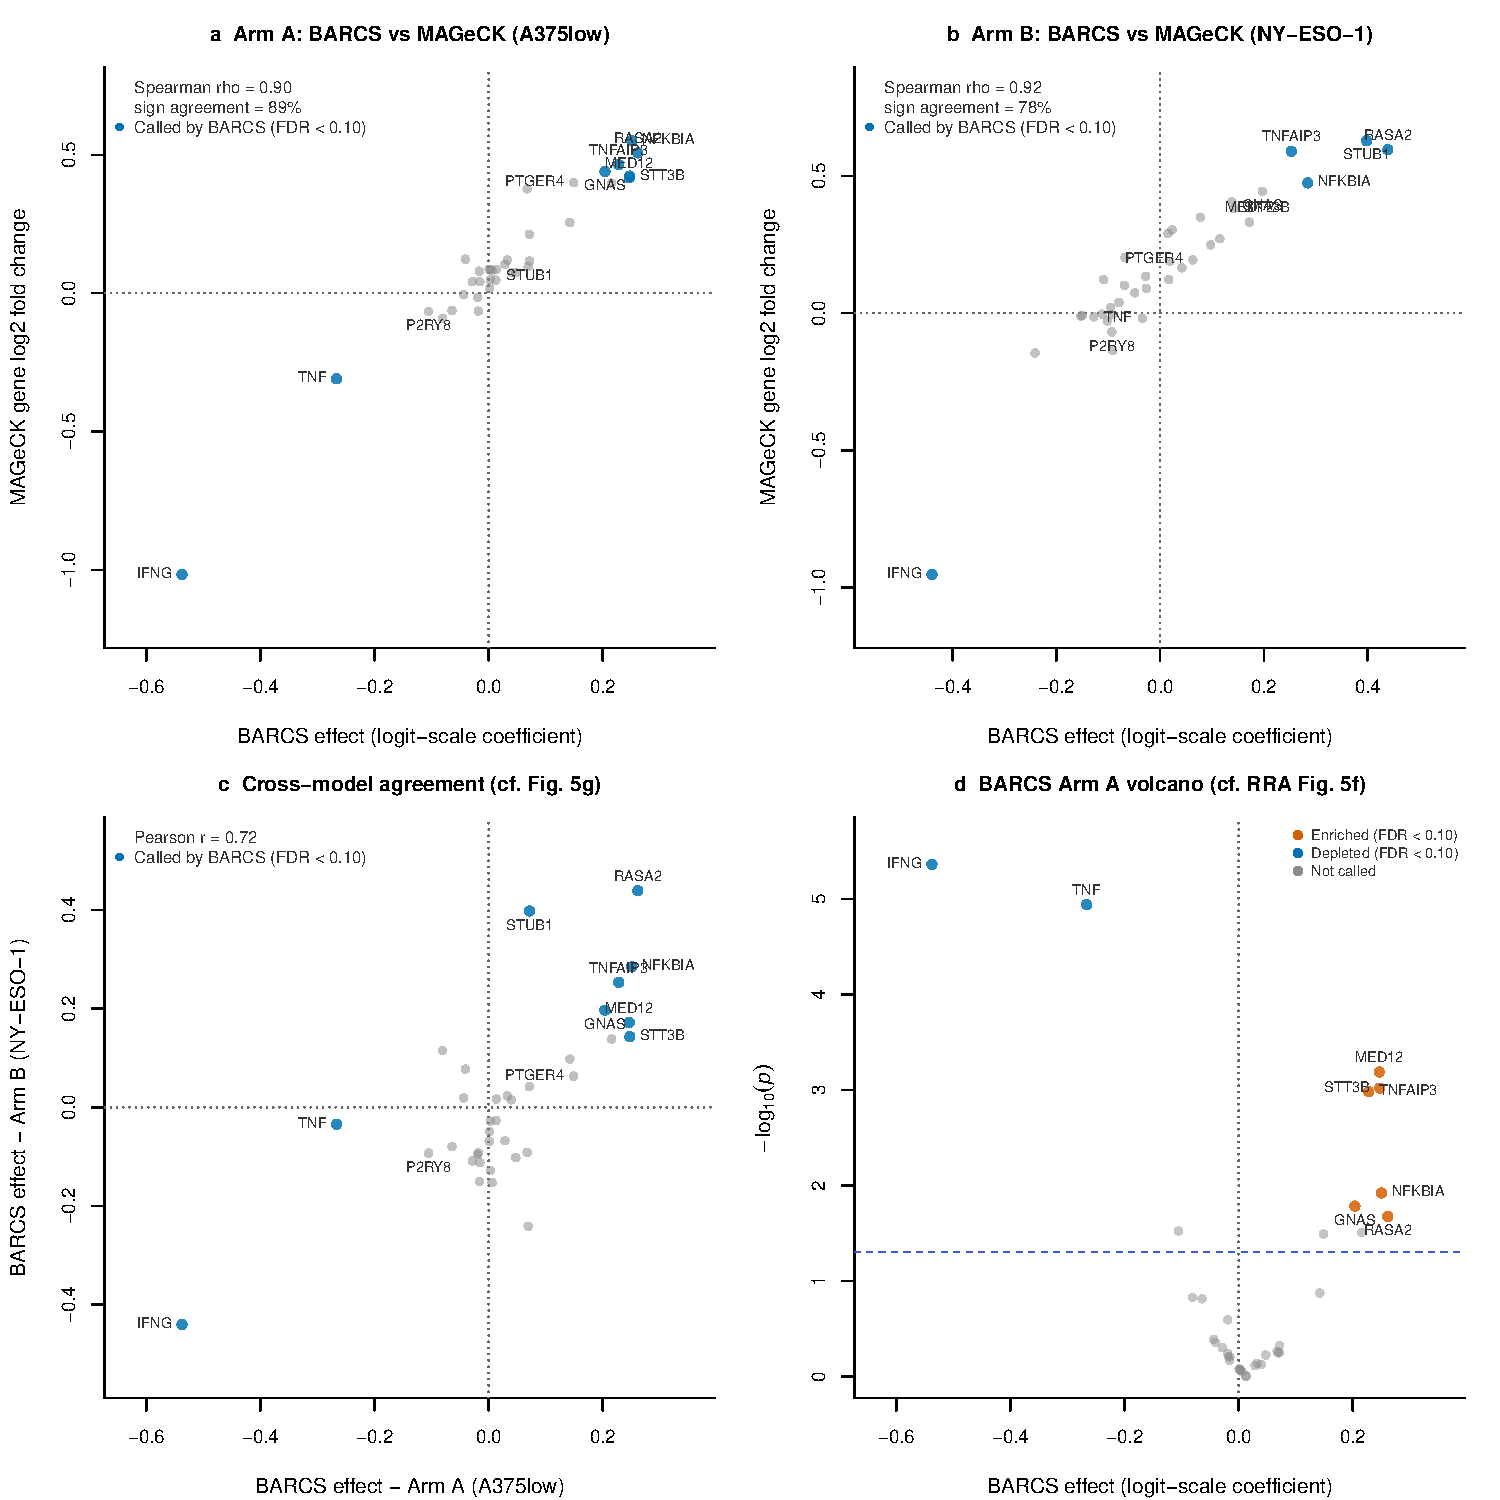
\includegraphics[width=\textwidth]{figures/liu_tcell_publication_comparison.pdf}
\caption{\textbf{BARCS re-analysis of the \citet{liu2026invivo} sub-library
IFN$\gamma$ screen against the published MAGeCK analysis.}  (a,~b) BARCS
gene-level effect versus the published MAGeCK gene log$_2$ fold change for Arm~A
(A375\textsuperscript{low}) and Arm~B (NY-ESO-1); blue marks genes called by
BARCS at FDR $<0.10$.  BARCS reports a logit-scale coefficient and MAGeCK a
log$_2$ fold change, so the panels are read as sign and rank concordance
(Spearman $\rho=0.90$ and $0.92$), not as a fitted slope.  (c) BARCS Arm~A versus
Arm~B effects, the cross-model agreement shown with RRA scores in the paper's
Extended Data Fig.~5g ($r=0.72$).  (d) BARCS Arm~A volcano, the counterpart of
the MAGeCK RRA volcano in Extended Data Fig.~5f; enriched and depleted calls at
FDR $<0.10$ are coloured and the dashed line marks $p=0.05$.}
\label{fig:liu}
\end{figure}

\FloatBarrier
